\documentclass[english]{cpp-hmwk}
\usepackage{blindtext}

\begin{document}
\Homework{Lindenmayer systems - a flexible C++ implementation}{Steffen Knoblauch}

\begin{abstract}
Lindenmayer Systems, short L-systems, are the result of research from Lindenmayer et al.\cite{prusinkiewiczp.lindenmayera.2004} about the geometric features of plants.
L-systems are a concept to mathematicaly/formal describe and model the growth processes of plant development. They are not only restricted to the plant based developments, but can also be used to generate fractals.

L-systems have an inital state and use rules, like a formal grammar, to transform or rather rewrite the current state to create the next state of the development from a plant or a fractal.
Therefore it is possible to successive calculate each state of the development.
This state can be interpreted as commands for a turtle graphic, which creates the opportunity to draw the created fractals or plant states. 

Goal of this paper is to design an architecture for L-systems, which includes an implementation for L-systems, their calculation and an interface for a turtle graphic. The interface should enable the polymorphic use of different turtle graphic implementations and enable drawing of a state.
\end{abstract}

\pagebreak
\section{Introduction}
L-systems are a formal way to describe plant or fractal development and interpret the result as a graphic. This paper aims not only to provide an overview of Lsystems, but also includes the discussion about the architecture and is organised as follows. Section \ref{section:lindenmayer} briefly introduces the general idea,  based around object rewriting, the grammar of L- systems and the interpretation of a L-system as graphic.
After discussing the architecture and possible implementation steps, a final concept for an implementation is proposed. The code for this implementation is available via a github repository.\footnote{See https://github.com/frozzenshooter/LSystems}

The remainder of the paper provides some examples and a conclusion with future enhancements.

\section{Lindenmayer systems}
\label{section:lindenmayer}
\subsection{History}
\label{section:history}
''[L-systems] were introduced in 1968 by Lindenmayer as a theoretical framwork for studying the development of simple multicellular organisms [...]'\cite[Preface, p.~VI]{prusinkiewiczp.lindenmayera.2004} and were later used in computer graphics to generate visuals of organisms and fractals.

In the beginning the focus of L-systems theory was based on larger plant parts and the graphical interpretation used chains of rectangles to display a L-system. Further research into L-system resulted in new interpretations and extensions. For example an interpretation of a L-system state with a LOGO-style Turtle. These extensions make it possible to model more complex plants and fractals and display them in a graphical way. \cite[Cf. Chapter 1.3, p.~6]{prusinkiewiczp.lindenmayera.2004}.

\subsection{General idea}
\label{section:gerneralidea}
The use of a rewriting system, based on a formal grammar, is the general idea of a L-system. The shape of a plant or a fractal consists of geometric pieces, for example a branch of a tree has several subbranches. ''When each piece of a shape is geometrically similar to the whole, both the shape and the cascade that generate it are called self-similar.''\cite[Chapter 6, p.~34]{benoitmandelbrot1982} The self-similaritiy makes it possible to create a formal description for the plant or fractal generation as a formal grammar, further discussed in section \ref{section:grammar}. Rewriting uses this formal description to generate the diffferent states of the development. ''In general, rewriting is a technique for defining complex objects by successively replacing parts of a simple initial object using a set of rewriting rules or productions.''\cite[Chapter 1.1,  p.~1]{prusinkiewiczp.lindenmayera.2004}. 

This concept can be used to rewrite an inital string, called axiom, with specific rewriting rules.
A simple example is the following grammar, which consits of only two nonterminals, A and B, and two productions. 
The first production is A\rightarrow AB, the second one is B\rightarrow A. The arrow '\rightarrow' symbols the replacement, the rewriting, of the object on the left with the object on the right of the arrow.
The L-system has as axiom the value 'A' and will be expanded with these rules, creating the results in figure \ref{figure:simple_lsystem}.

\begin{figure}[h!]
	\centering
	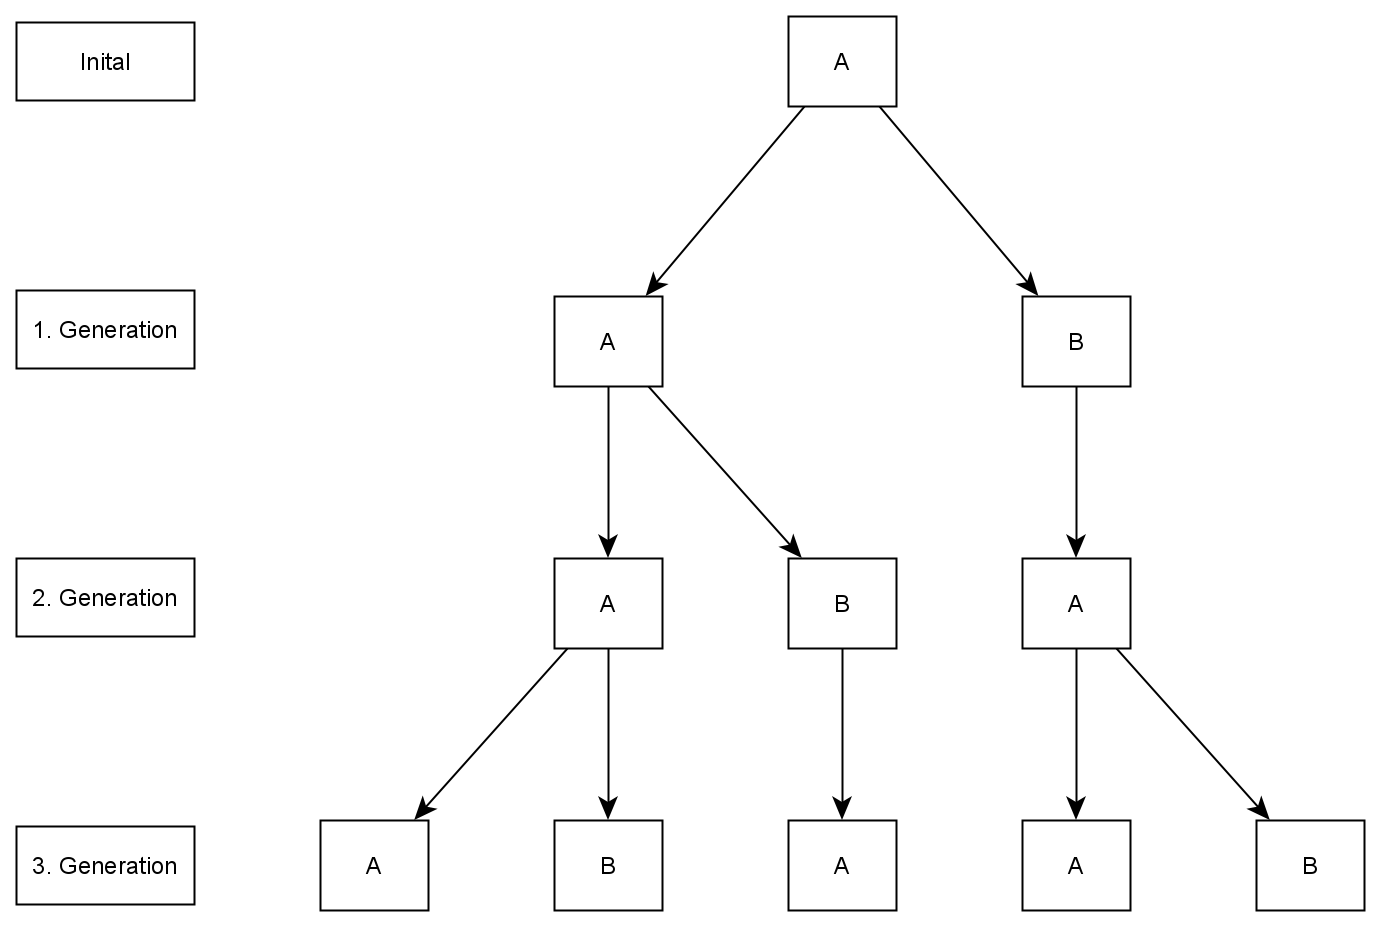
\includegraphics[width=0.7\columnwidth]{../graphs/Examples/simple_lsystem.png}
	\caption{Simple L-system}
	\label{figure:simple_lsystem}
\end{figure}

As first step, using rule one, the nonterminal A is replaced with AB, resulting in the first generation. The result of the first generation process ('AB') will be used to determine the second generation. For all nonterminals the productions can be parallel applied. In this case, the nonterminals A and B will be replaced, because both have existing productions. This results in the second generation with 'ABA' as result.

This process can be successively and recursively repeated for an arbitrary amount of generations and create a fractal or plant with self-similar parts. The more generations are calculated, the more detailed is the resulting state. 

\subsection{Grammar}
\label{section:grammar}
The definition of an L-system can be done similar to a Chomsky grammar, but there are some general differences. In Chomsky grammars, the productions are applied sequentially, whereas in L-systems they can be applied parallel. This has some consequences for the formal properties of an L-system, for example a context-free L-system can produce a language which cannot be produced by a context-free Chomsky grammar.\cite[Cf. Chapter 1.1, p.~3]{prusinkiewiczp.lindenmayera.2004}

\noindent This paper will only focus on a class of L-systems, the DOL-systems, which can be used for string based rewriting systems. This class is deterministic (D) and context-free (O) and can be formaly described  by a tuple:

\begin{center}
G = (V, $\omega$, P)
\end{center}

V: set of symbols as alphabet of the L-system - consisting of terminals and non terminals

$\omega$: axiom - nonempty word of the alphabet, which should contain at least one nonterminal

P: set of productions

\medskip
\noindent A production consists of a predecessor, a nonterminal symbol of the alphabet, and a successor, the replacment of the nonterminal in the next generation.
To guarantee the deterministic characteristic of a L-system, it is relveant that there is only one production for each nonterminal of the alphabet.The identity production is implicit a part of the set of productions.\cite[Cf. Chapter 1.2, p.~4f.]{prusinkiewiczp.lindenmayera.2004}

\medskip

If in the process of rewriting a terminal symbol is found, there will be no explicit production applied, but rather the identity production is applied. Terminals will therefore remain in future generations and won't extend the result further.

\medskip

\noindent As mentioned in section \ref{section:history} there are other extensions of a basic L-system. The extensions introduce more possiblities for the generation process, like a non-deterministic behaviour. These extensions result in new grammars, which can represent more complex plants or fractals:

\begin{itemize}
\item Stochastic grammars: the system isn't deterministic anymore, because there can be multiple productions with a probaility for the same nonterminal, which results in a randomisation of the generation
\item Context senstive grammars: productions don't only look for the nonterminal, they rather look for the symbols bevor and after the current symbol to process, the context
\item Parametric grammars: it is possible to set additional parameters for a symbol to influence the generation or the evaluation of the data
\end{itemize}

\subsection{Interpretation as turtle commands}
\label{section:turtle}
The L-systems introduced to this point are capable of creating a string, based on a grammar. In order to create a graphic of a L-system state, this state can be interpreted as commands of a turtle.

\noindent A turtle is a concept introduced by the language Logo as a tool for computer graphics.\cite[Cf. Chapter 10, p.~179]{harvey1997computer}

\noindent A state of a turtle can be described as a tuple\cite[Cf. Chapter 1.3, p.~6ff]{prusinkiewiczp.lindenmayera.2004}:

\begin{center}
S = (x,y, $\alpha$)
\end{center}

x and y are Cartesian coordinates

$\alpha$ is the direction in which a turtle is facing, called heading

\medskip

\noindent A turtle can move in the Cartesian coordinate system by altering the current state. It is possible to think of it as a real turtle with a pen attached to it, walking on a paper. While moving thourgh the coordinate system or the paper, the turtle can draw lines. Given that, the turtle can receive different commands. The commands let the turtle walk on the paper or the coordinate system by altering the current state and drawing a line. For now it will be restricted to a two dimensional coordinate system, but it is also possible to enhance it for a three dimensional coordinate system.

\medskip

\noindent The walking path of the turtle is controlled by commands. Therefore, a defined step size \textit{d} and an angle \textit{$\theta$ } is needed to calculate the next state of the turtle. These general commands are offered from a turtle: \cite[Cf. Chapter 2]{goldman2004turtle}

\begin{itemize}
\item Draw: moves one step in the current facing direction drawing a line 
\item Move: moves one step in the current facing direction without drawing a line
\item Right-turn: turns to the right by the angle $\theta$
\item Left-turn: turns to the left by the angle $\theta$
\end{itemize}

\noindent Additional tothe turtle state, with postion and facing direction, there is a state for the pen. The pen state is part of a turtle and consist for example of a color and or a line width.

\medskip

\noindent  The explained turtle concept makes it possible to interpret the result of a L-system. Therefore, a mapping between the symbols in the alphabet and the commands, which should be executed, is needed.
This could be done by an arbitrary mapping between a nonterminal or a terminal and a command. For this paper the following mapping will be used, but the concept for the architecture includes the possibility to use other mappings in the future.

\noindent Alphabet V,  a basic version of a L-system, is used for the mapping:

\begin{center}
V = (F, f, +, -)
\end{center}

This alphabet will be mapped with these turtle commands:

\begin{center}
\begin{tabular}{ c l }
Symbol & Turtle interpretation \\
\hline
F & Draw a line in the facing direction  \\ 
f & Move in the facing direction  \\  
+& Turn right  \\  
-& Turn left  \\  

\end{tabular}
\end{center}

\noindent This interpretation enables to draw the result of the L-system by iterating over every terminal and nonterminal of the result state and calling the mapped command. If no command is mapped the symbol will be skipped.

\subsection{Examples}
\label{section:examples}
This section will present some examples for L-system grammars which create fractals. They were created with the implementation described in section \ref{section:impl}, under the use of the command mapping from section \ref{section:turtle}. 
\footnote{The grammars and further examples can be found under: \fullcite{examples1997}}
  
\subsubsection{Hilbert curve}
This fractal will be generated with the simple axiom 'L' and tow productions: 

\begin{itemize}
\item L\rightarrow +RF-LFL-FR+
\item R\rightarrow-LF+RFR+FL-
\end{itemize}


\noindent The turtle will be initalized with an angle of 90° and length \textit{d} = 5 for a single step. The result is displayed in figure \ref{figure:Hilbert}.

\begin{figure}[h!]
	\centering
	
\includegraphics[width=0.6\columnwidth]{../graphs/Examples/hilbert.png}
	\caption{Hilbert L-system - 7 generations}
	\label{figure:Hilbert}
\end{figure}
 

\subsubsection{Sierpinski triangle}
This fractal will be created with 'F' as axiom and two productions:

\begin{itemize}
\item X\rightarrow YF+XF+Y
\item Y\rightarrow XF-YF-X
\end{itemize}

\noindent The turtle will be initalized with an angle of 60° and length \textit{d} = 3 for a single step. The result is displayed in figure \ref{figure:Sierpinski}.
 
\begin{figure}[h!]
	\centering
	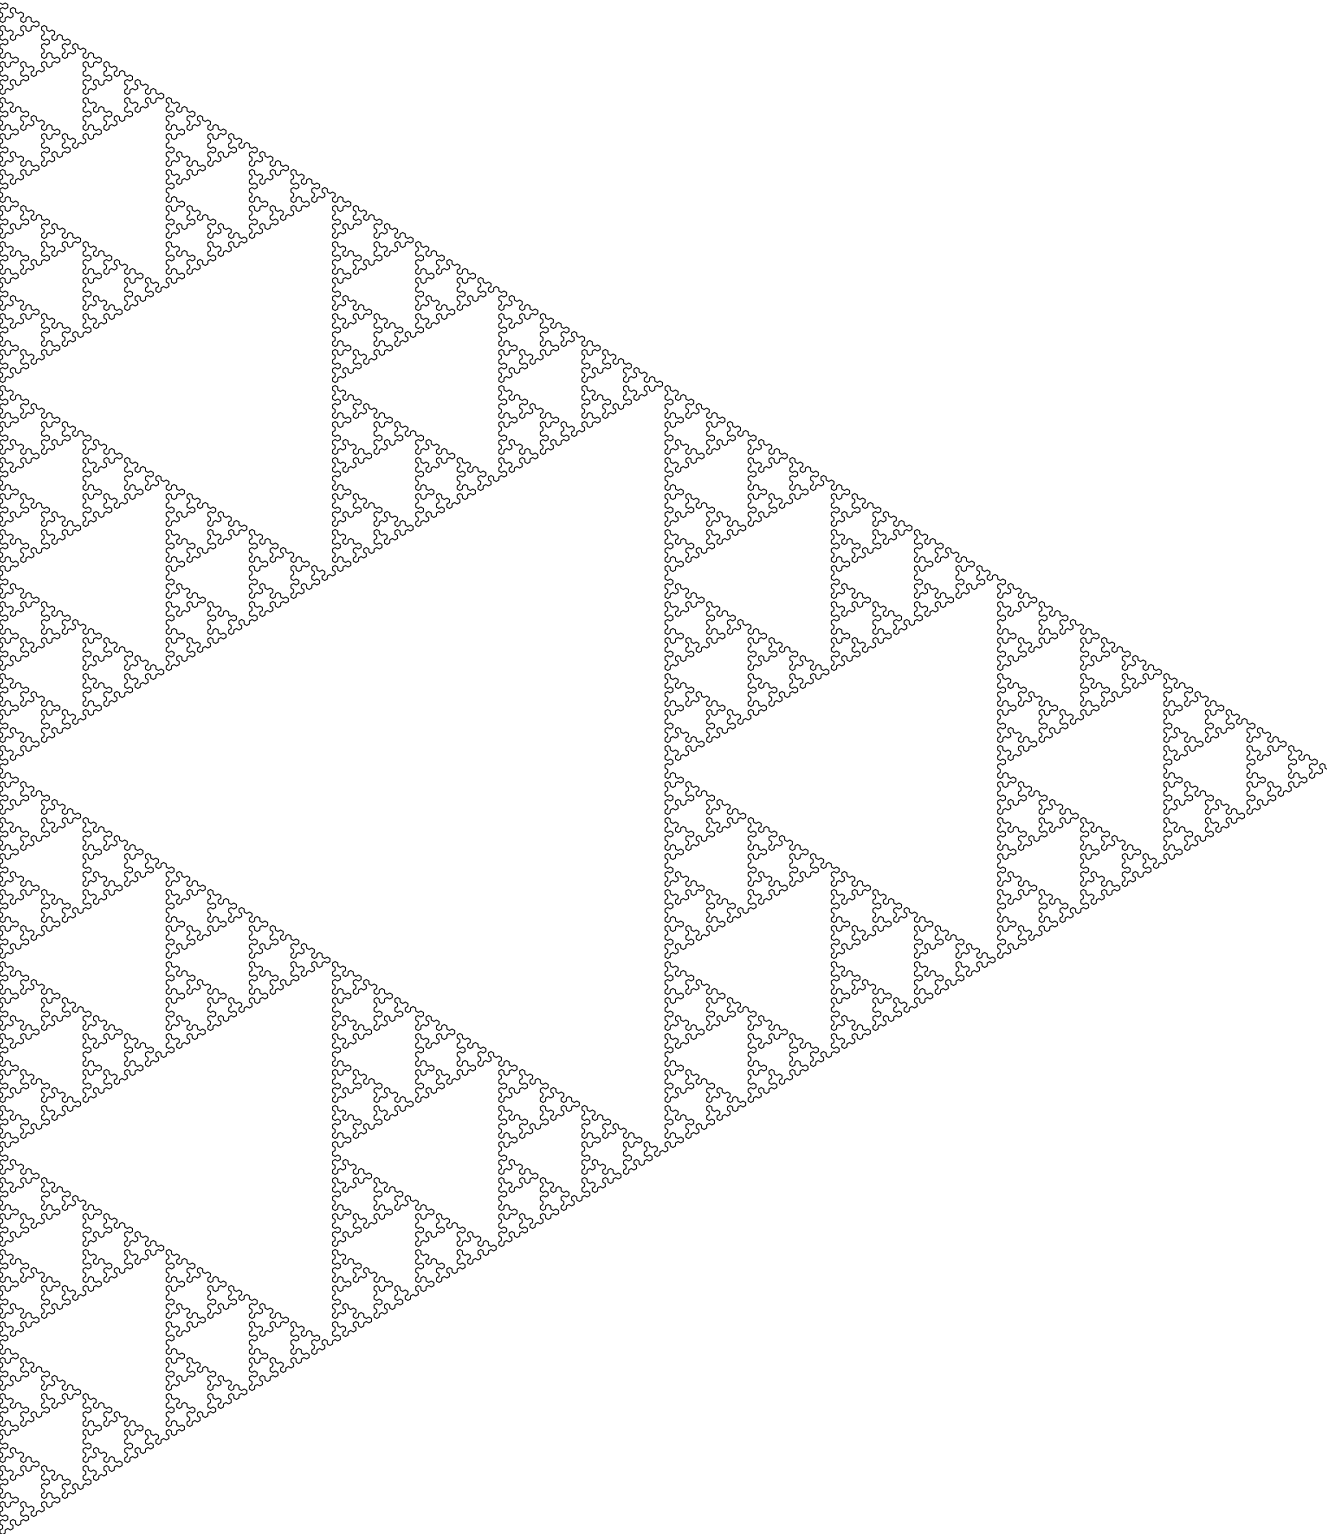
\includegraphics[width=0.6\columnwidth]{../graphs/Examples/sierpinski.png}
	\caption{Sierpinski L-system - 9 generations}
	\label{figure:Sierpinski}
\end{figure}
 

\clearpage
\section{Architecture}
The primary goal of this paper is creating an architecture and an implementation of a L-system as described in section \ref{section:lindenmayer}. The focus of the architecture will be on flexibility and expandability and therefore is the following section splitted into several parts with discussions about different aspects of the final architecture.

\subsection{Requirements overview}
The architecture for a L-system, as introduced in section \ref{section:lindenmayer}, has several requirements. This section will introduce the needed core requirements for an architecture with a flexible L-system and turtle.

\medskip
\noindent The core of the concept is the L-system itfself, which is the base to guarantee a flexible use. The L-system holds relevant data like the grammar, consisting of productions and an axiom. The L-system should offer a way to configure a grammar and guarantee the usage in different architectures, without hardcoded grammars. The L-system has to be able to successively generate the next states with configured grammar and grant access to this generated result.

\medskip

\noindent The turtle is another key component, which will be used to interpret the result of a L-system. The turtle has to offer the typical turtle commands as introduced in section \ref{section:turtle}. In order to provide a turtle that is as extensible as possible, it should be possible to implement it flexibly. Therefore an interface should be offered, that enables a fast exchange of implementations. Depending on the implementation of a turtle, it should be possible to configure the turtle and change properties, like the color or line width.

\medskip
\noindent A mapping between the turtle commands and the L-system alphabet is an important part, so it is possible to call the correct turtle commands. In order to create an image of a plant or a fractal development state, it is required that the mapped commands get called, after interpreting the L-system result.


\subsection{L-system}
\label{section:lsystem_discussion}
This section provides a dissussion of possible implementations of the L-system and a final proposal.

\medskip

\noindent A simple and rather naive idea would be an object which holds the L-system as a string and addtional the grammar, consisting of productions and an axiom. This L-system could offer a function that calculates the next generation by iterating over every char in the string. If there is a production for the current char, the char will be replaced according to the production with the successor. This function could be called for n generations to create the n-th generation of the L-system, as show in figure \ref{figure:naive_lsystem}.

\begin{figure}[h!]
	\centering
	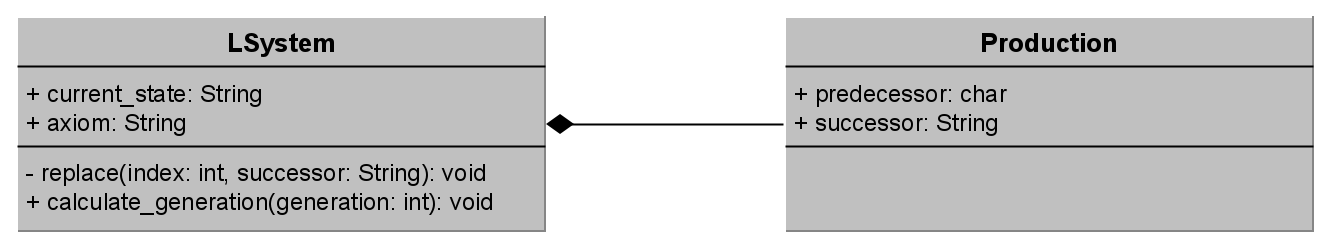
\includegraphics[width=1\columnwidth]{../graphs/LSystem/naive/class_diagram_l_system_naive.png}
	\caption{Naive L-system}
	\label{figure:naive_lsystem}
\end{figure}

\medskip
\noindent This idea has several design flaws resulting in a bad performance and unflexible architecture. The first flaws exist because of the lack of seperation between datastructure and processing of the data. It is not possible to simply exchange the datastructure or the function without the seperation, which affects flexibility of the L-system negative. This can be solved by extracting the functionality into a seperate function and the datastructure remains as ''dumb'' object. The seperated function can be a used to manipulate the current state in the datastrutcture itself and also creates the opportunity to exchange the underlying datastructure, as long as the datastructure fullfills some formal properties, like the support of access to the string and grammar.\newline
For a more flexible design additional changes could be done, because the current idea bases on chars as alphabet of the grammar. The L-system could be enhanced by allowing arbitrary objects as symbols of the alphabet, as long as they provide certain functions, like a operator to compare them. Instead of a string, the objects could for example be saved as a list.\newline
A further flaw is the bad performance, because of the use of a string to save the current state/generation. There are two reasons why the performance is bad, especially for larger generations. The first reason is the size of the string itself, which will grow very fast because of the nature of a L-system. Every nonterminal will be often replaced by severall symbols, which enormously increases the total size of the string for each generation. Additional to the large amount of space needed for the string, the replace in a string needs to be done for each nonterminal, which can result in a big overhead. Because of this problems, another more efficient design is needed.\newline
This implementation only works for simple L-systems where only a few generations are needed.

\medskip
\noindent In order to solve this problems and to create a more efficient and flexible architecture, let's recap the nature of L-systems. The generation of a L-system is based on a rewriting process. This process iterates over every object in the current state and calcualtes the resulting generation by applying the productions. Because of the restriction to DOL-systems, the rewriting is not context-sensitive and can be done independent from other objects of the current state. If a object gets replaced by the successor of the production, the result of this replacment can be handled independent. Consequently, the calculation of the n-th generation can be done for each object on their own and can simply be done in a recursive manner.\newline
There is only a limited number of productions in a grammar of a L-system. Each of these productions is choosen deterministic when comparing the current nonterminal with the predecessor. The next generation is created by rewriting the current state, when a nonterminal is often in the current state, the same production can be used. If the same production is used muliple times, the resulting generation has a lot of similar objects or more specific the same string muliple times. The repeating data and the recursive calculation can be used to improve the naive idea.

\medskip
\begin{figure}[h!]
	\centering
	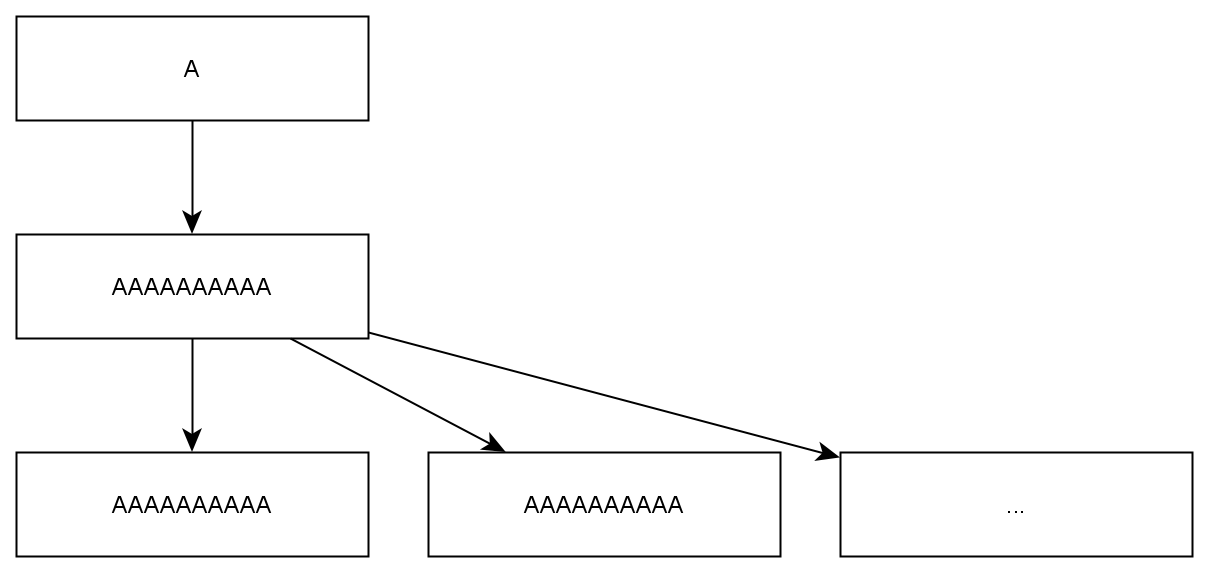
\includegraphics[width=0.8\columnwidth]{../graphs/LSystem/examples/simple_grammar_data_doubling.png}
	\caption{Memory reduction}
	\label{figure:lsystem_mem_reduction}
\end{figure}

\noindent The simple example in figure \ref{figure:lsystem_mem_reduction} shows the possible reduction of data using the following grammar:

Axiom: A

Production: A \rightarrow AAAAAAAAAA 

\medskip
\noindent This rather ideal example shows how it would be sufficient to save just parts of the resulting string to represent the whole generation of a L-system. For this example it could be possible to save ''AAAAAAAAAA'' and how often it is needed. Because of the repetitions, this is partly even for more complex grammars possible.

\medskip
\noindent With this knowledge multiple improvements can be discussed. The first possible improvement is storing the data not in a simple list, like a string, but instead in a more sophisticated datastructure. For this case a graph as datastructure is better suited. Such a graph enables a better performance for replacements and reduction of memory space.

\medskip
\noindent The graph has a special sturture to achive the improvements for a L-system. The following grammar is used to demonstrate the possible improvements:
 
Axiom: A

1. Production: A \rightarrow BBB

2. Production: B \rightarrow AAA

\medskip

\noindent A natural improvement of a graph is the replace function. This could be done by simply creating new childnodes with the replaced data. In figure \ref{figure:lsystem_graph} is a example with the given grammar. Each generation has its own nodes with data of the current state. A level of this graph represents a whole generation and can be accessed with the depth of the nodes.

\begin{figure}[h!]
	\centering
	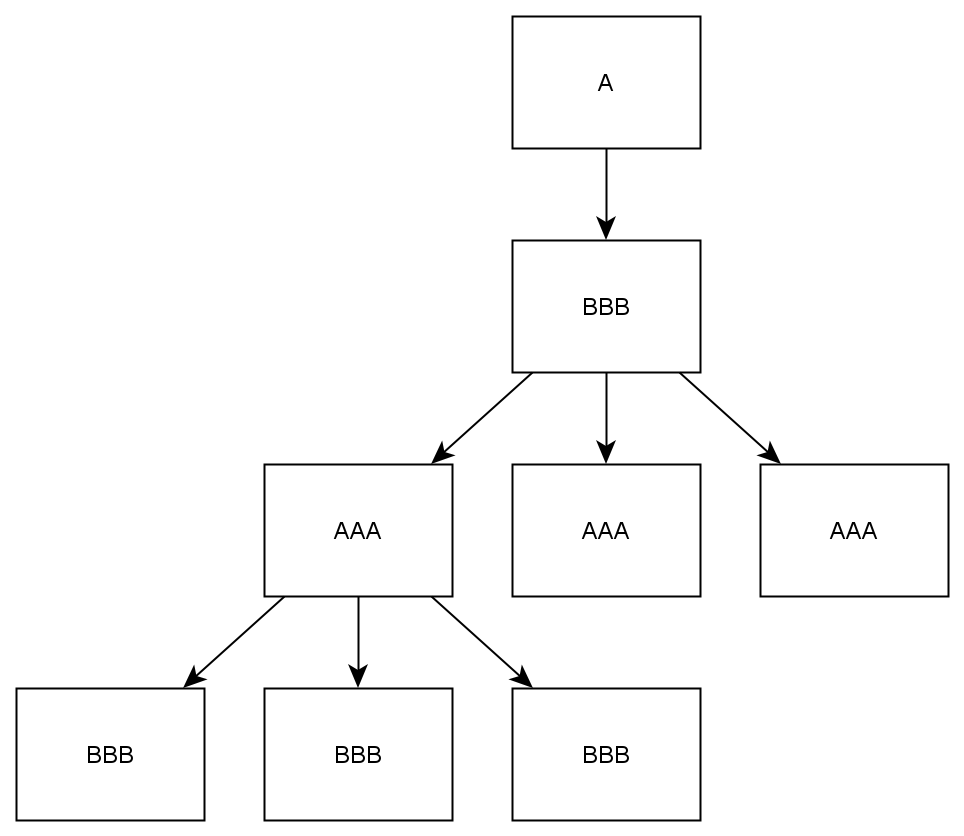
\includegraphics[width=0.8\columnwidth]{../graphs/LSystem/examples/lsystem_graph_example.png}
	\caption{L-system as graph}
	\label{figure:lsystem_graph}
\end{figure}

\medskip

\noindent This graph still has the problem of the redundant data, because every note contains its own data. For example in the second generation the part ''AAA'' is stored three times. This can be improved with another indirection of the data. This concept results in a datastructure containing a graph to store the dependencies and a container for the data itself. In figure \ref{figure:lsystem_graph_mem_reduction} is an example for this indirection. Each node saves a pointer or id of the data it represents. In this graph a replace could also be done with the creation of a childnodes.

\begin{figure}[h!]
	\centering
	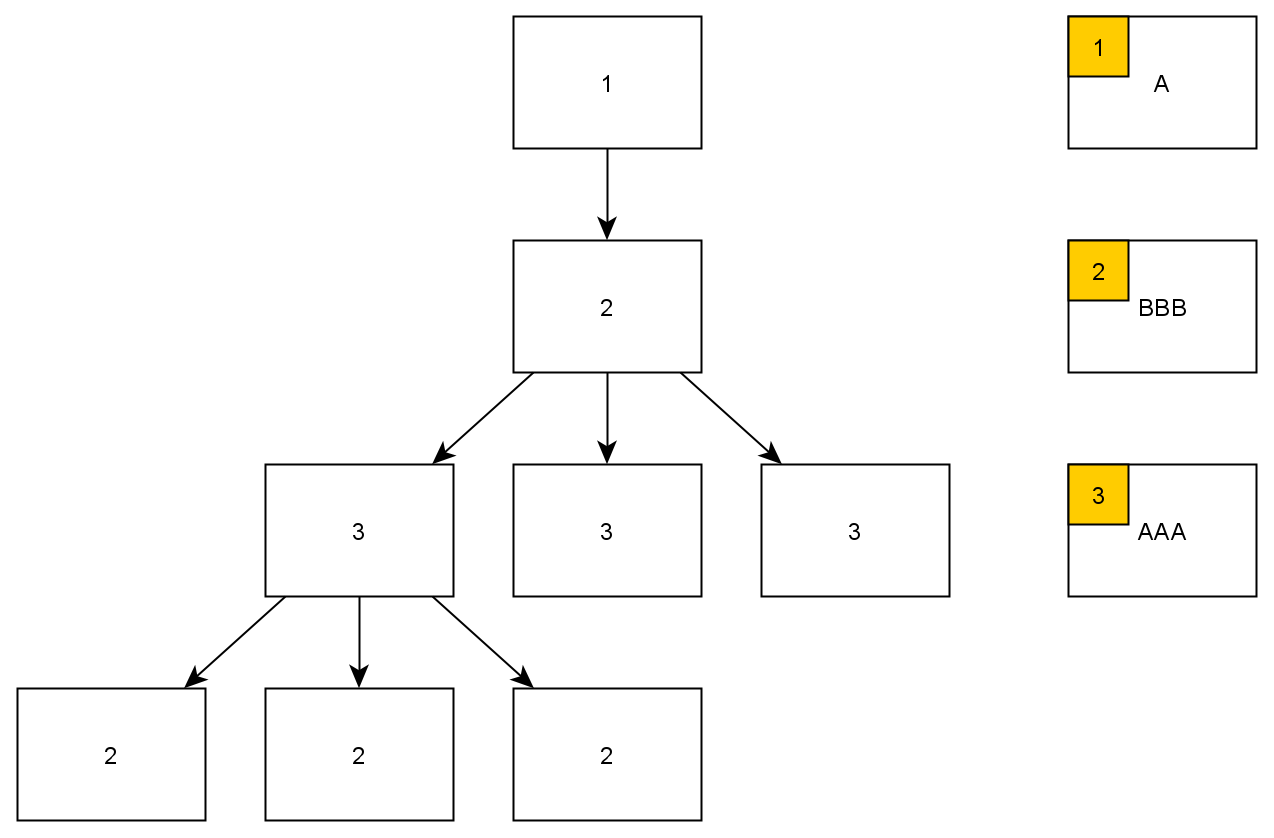
\includegraphics[width=0.8\columnwidth]{../graphs/LSystem/examples/lsystem_graph_reduced_example.png}
	\caption{L-system as graph with improved memory consumption}
	\label{figure:lsystem_graph_mem_reduction}
\end{figure}

\medskip
\noindent Both of the described graphs hold every calculated generation, which allows the access to an arbitrary generation with the restriction to the deepest calculated generation. To reduce the amount of storage needed even more, it is possible to neglect if all generations are needed or only the current generation. If only the last calculated generation is needed, the graph can be simplified even more. To discuss the simplification, it is necessary to look further in the different ways to do the replacement. It  is possible to iterate over the node data and replace for each symbol of teh data at a time. For example with the current grammar the data ''AAA'', could be replaced by replacing each ''A'' at a time. Because of the focus of DOL-Systems, another possible method is to replace a node with all childnodes at once.\newline
There seems to be no difference, but in combination with the proposed next step of the graph, it is relevant. If not all generations have to be stored, it is possible to remove a completely replaced parentnode. For example in figure \ref{figure:lsystem_graph_one_generation}, it is not needed to save the crossed out nodes, because they are completely replaced. In this simple example is it already possible save only four instead of six nodes and reduce the data. This results in a flat graph with only a few nodes depth, but only the current state of a L-system. For this graph, it is  important how the replacement is done. If the replacment is done with the all at once method, the parent node can be deleted directly. If the step by step replacement is done, it is nessecary to alter the parentnode data for each replacement. Only when the complete data and the parentnode is replaced, this node can be deleted. The complete replacement is simpler to implement, because the altering of parentnode data is not needed.

\begin{figure}[h!]
	\centering
	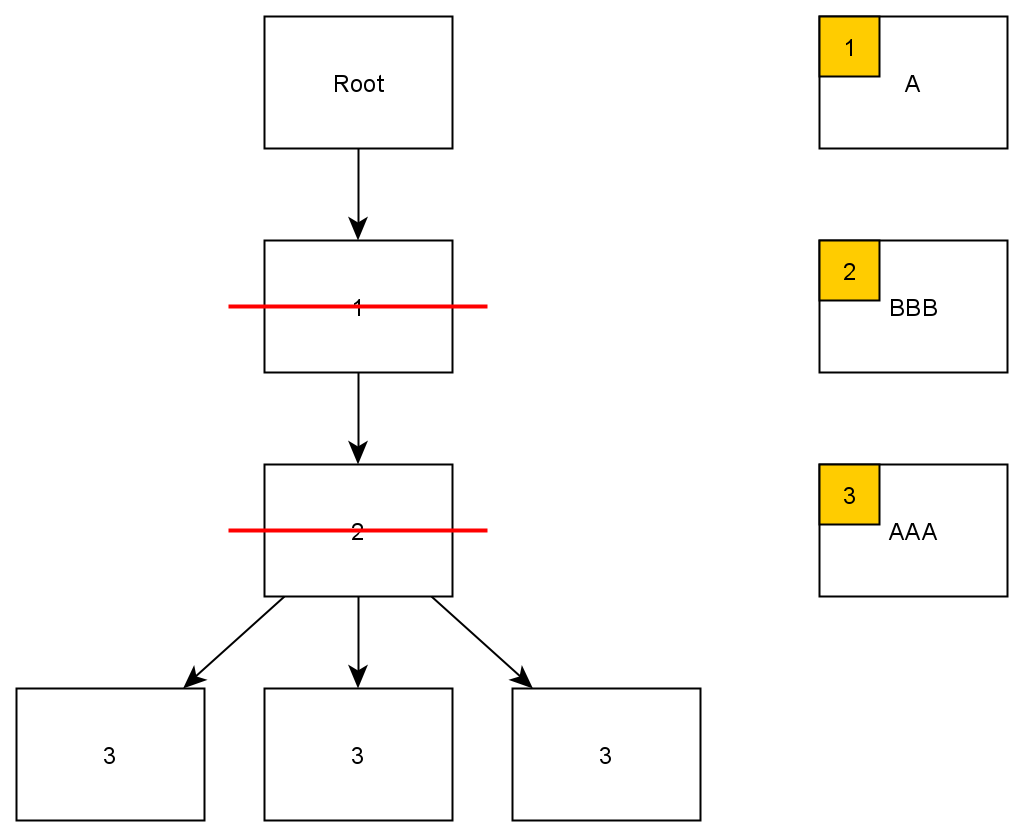
\includegraphics[width=0.8\columnwidth]{../graphs/LSystem/examples/lsystem_graph_reduced2_example.png}
	\caption{L-system as graph with one generation}
	\label{figure:lsystem_graph_one_generation}
\end{figure}

\medskip
\noindent A graph is as consequence a faster and memory saving approach in comparison to the naive L-system.

\bigskip

\noindent Another possible simplification is to neglect storing the generations of a L-system at all. Instead of saving the generation of a L-system in a datastructure, the result can be calculated on demand and never stored. The only data such a L-system would hold, would be the grammar itself. The calculation can be done with a recursive function, that will return the generation. Clearly an advantage is the reduction of needed storage space, but this reduction is only achived at the cost of recalculation for each generation. Whenever a generation is needed, it is nessecary to calculate again and it is not possible to use a previous result.
If a generation is needed multiple times or if it is needed to setp forwards and backwards in the result, a solution could be to store the result in another object. This calculations also guarantees a flexiblity, because you can either only calculate the generation once and use the result directly, like in this case to call the turtle commands, or save it for later usage.
 
The recursive function can be designed flexible in order to allow a simple exchange of a L-system datastructure. This results in two main components, the L-system datastructure and the function, which accepts a L-system datastructure and calculates the generation. The L-system, which the function receives, has to fullfill some requirements, like to offer access functions. This will be described in further detail in the implementation in section \ref{section:impl}.
 
\bigskip
 
\noindent There are the two possible ways to handle the L-system. The storage as a datastructure, based on a graph, and the recursive calculation. For this paper, it is completely sufficient to calculate the generation on demand, because it is only necessary to call the turtle command once for each object of the L-system generation. As consequence no implementation of the graph is needed. Other use cases in the future might need to store the data. This would even be possible with the recursive function, when the result is stored in another object, for example a graph. The proposal for the L-system is shown in figure \ref{figure:lsystem_proposal}.

\begin{figure}[h!]
	\centering
	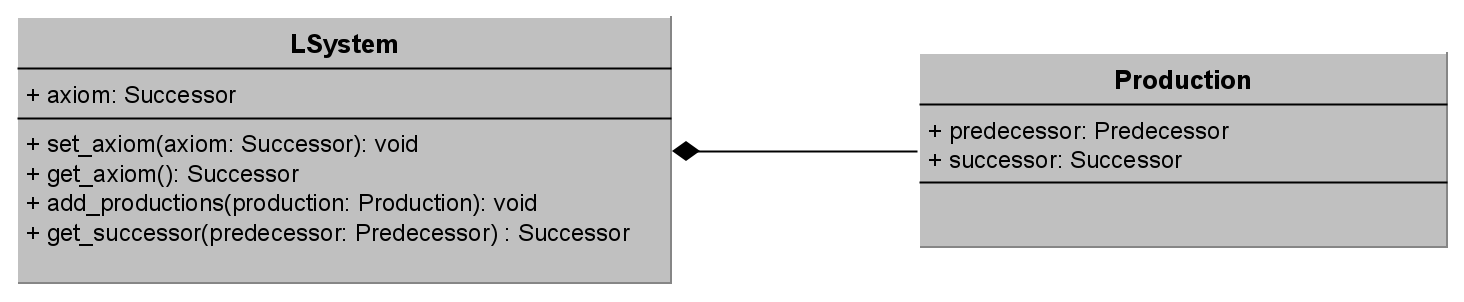
\includegraphics[width=1\columnwidth]{../graphs/LSystem/examples/l_system_proposal.png}
	\caption{L-system proposal}
	\label{figure:lsystem_proposal}
\end{figure}

\medskip
\noindent The proposed L-system will just hold the grammar for a L-system, which will be given to the recursive function. This L-system can be used in a flexible way, because it can be configured without a restriction of the grammar.Additonal, there is only a general type restriction for the axiom and the prodcutions. The types called Successor and Predeccessor can be choosen freely, but they need to fullfill formal requriements. The self-similarity and ergo the rewriting need to be represented by the types. The Successor type must consist of Successor objects itself, which can be splitted into objects of the Predecessor type. Each Predecessor object must be comparable to another Predecessor to be able to rewrite the L-system. 
 The type of the axiom and the successor have the same type, in order to guarantee that they are splittable in smaller parts.
 
To this point the discussion doesn't include how the turtle commands can be called. As already mentioned there must be mapping between the commands of turtle and the alphabet of the L-system. The mapping will be discussed further in section \ref{section:turtle_mapping} and for now we just asume a mapping exists in some way. When using a graph, it would be possible to call the turtle commands by accessing a generation data and interpret the objects.

Here the implementation is based on a recursive function. This function can call the turtle commands for a generation or more specific when the recursion depth is reached. How this will be done in detail is described in section \ref{section:impl}, but is based around the idea of an output iterator. The recursive function will receive an arbitrary output iterator and instead of interpreting the data in the function itself it will just hand over the objects of the generation to the iterator. This iterator can than interpret the objects as turtle commands and call them. The iterator has no restrictions on what to do with the data. For example the iterator may be used to save data in an arbitrary datastructure or print it in a file.

Overall allows this concept, consiting of the L-system datastructure and the recursive funtion, a possible user a flexible field of operation. The recursive function and the L-system datastructure can be used completely independent. For this concept, these components will be used together, in combination with other components, like a turtle and a turtle command mapping.

\subsection{Turtle}
A quiet important component of the architecture is the turtle. The turtle has to offer the typical commands as described in section \ref{section:turtle}. A turtle should be so flexible that it is possible to implement it for different Framworks, for example OpenGL or the Cairo graphics library. An abstract interface, with a minimal set of commands, will allow to implement this. A turtle like this is not only bound to a special graphics framework, but can be even implemented for other usecases, like generating text on the console or a file.
The most general or abstract version of a turtle offers the four minimal functions of a turtle, as shown in figure \ref{figure:minimal_turtle}.

\begin{figure}[h!]
	\centering
	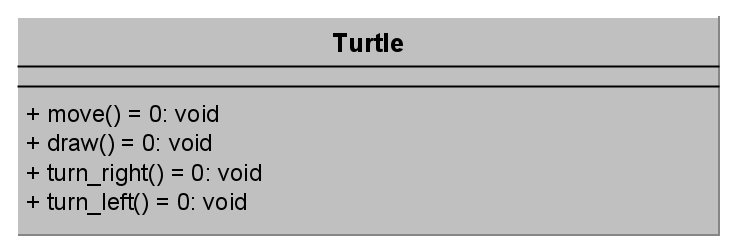
\includegraphics[width=0.6\columnwidth]{../graphs/LSystem/examples/class_simple_turtle.png}
	\caption{Minimal turtle}
	\label{figure:minimal_turtle}
\end{figure}

\medskip
\noindent More specialiced versions can offer more functions, depending on other needs and completly undependent of the paper usage of the turtle. For example an OpenGL implementation can offer more commands to represent a three dimensional turtle, like rotate around an axis. Additional to more commands, also different ways to configure a turtle can be offered for each specialization. Some possible implementations, in connection with this paper, will be described in section \ref{section:impl}.

Consequently the general interface is not only sufficient for this paper, but also for other usecases in the future.

\subsection{Turtle command mapping}
\label{section:turtle_mapping}
It is nessecary to map a command to an object in order to interpret the result of a L-system. As mentioned in section \ref{section:lsystem_discussion} a recursive function will be used to calculate the result of a L-system. Until this point we just assumed there was a mapping between the members of the alphabet of the L-system and the commands which will be called. In this scenario the recursive function receives an iterator, which can handle the generated data. 

The command mapping iterator is an example of an output iterator, which will handle data interpretation and calls of turtle commands. In figure \ref{figure:if_command_map} is the a concept of this iterator displayed , which will handle a L-system based on strings and chars. Such an iterator receives data, interprets it according to the mapping and calls the specified command.

\begin{figure}[h!]
	\centering
	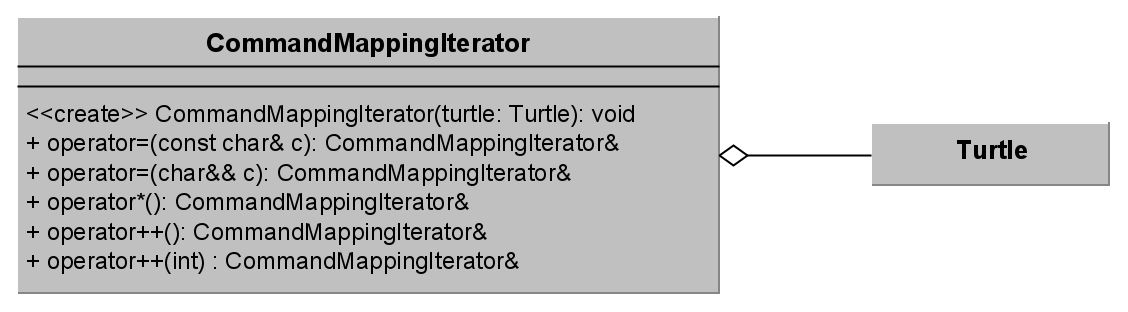
\includegraphics[width=1\columnwidth]{../graphs/LSystem/examples/class_command_mapping_iterator.png}
	\caption{C++ interface command mappin iterator}
	\label{figure:if_command_map}
\end{figure}

The recursive function will receive this iterator as parameter and just hands the result over to it. The command mapping iterator just has to select the mapped turtle command and call it.

The indirection in form of an iterator offers a clear separation between the calculation of the L-system generation and the handling of the data. In order to offer different mappings, new implementations of the iterator are nessecary. In the implementation, in section \ref{section:impl}, there is the implementation of the iterator example in figure \ref{figure:if_command_map} based on the grammar introduced in previous sections.

The architecture is not only restricted to iterators comparable to command mapping iterator, but every output iterator can be used to receive the data and handle it differently.

\subsection{Overview}
This section will now give a short overview of the disscuessed components and their dependencies. The general approach for the design was a flexible use of the separated components. It should be possible to use each component on their own and even exchange a component and still guarantee the functionlity. Under the premises, that exchanged components still offer the same functionality and data. In figure \ref{figure:overview} a simplified overview of the dataflow is illustrated. 

\begin{figure}[h!]
	\centering
	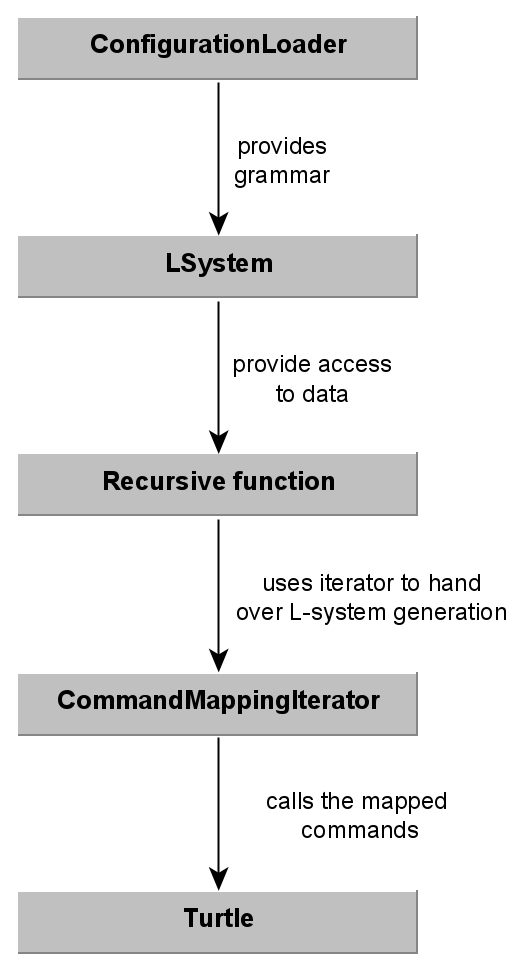
\includegraphics[width=0.4\columnwidth]{../graphs/LSystem/examples/overview.png}
	\caption{Simplified overview over the data flow}
	\label{figure:overview}
\end{figure}

At the beginning the L-system will be initalized. The L-system itself needs only to hold the grammar and and provide the access to it. The core of the L-system functionality is the recursive function, which will be used to calculate a L-system generation. This function offers a quiet flexible interface, because it should allow to use different L-system implementations, as long as the implementation provides a set of needed functions. These functions will be discussed in detail in section \ref{section:impl}. 
Another key part of the recursive function is the support of an arbitrary output iterator to hand over the calculated generation. This introduces not only a flexible usage of the function itself, but integrates well with already existing containers. 

The CommandMappingIterator is such an output iterator, which allows to use the provided interfaces to call the correct turtle command. Whenever data is handed over form the recursive function to the iterator, the iterator looks the data up and calls, if specified, the turtle command. The iterator here is  implemented for a determined mappping, but can be replaced by another implementation, as long as the implementation provides the typical output iterator functionality.

The final component is the turtle, which is used as abstract interface. This interface enforces the absolut minimal set of functions a turtle has to fullfill. Each spezialisation of a turtle has to independent handle their configuration and additonal dependencies.

As conclusion all the components can be exchanged with other objects, as long as they provide the needed interfaces. The needed interfaces will be described in detail in section \ref{section:impl} and addtional there are comments in the provided code.

\clearpage

\section{Implementation}
\label{section:impl}
This section provides the in detail description of the implementation for the components discussed in the previous sections. Addtional to the components other aspects of the implementation, like the build system are discussed.

\subsection{Build System}
\label{section:buildsystem}
The first important point for the implementation is the question what build system to choose or if a build system is even needed. A build system is needed or at least comfortable to use  because of two points. The first point is a fast way to build a complexer design and even extend it with libraries in a fast way. The second point, which also plays a big role for the question what build system to choose, is the choice of operating system.
 
A typical build system for C++ projects are Makefiles, which include a description what and how to build. The problem with Makefiles is the restricted support on Windows, which results in either an inconvenient setup or to choose another build system.
In this context CMake comes to mind, a generator for buildsystems. It is possible to define the project in a file and CMake can generate files for different build systems, on different operating systems. These resolves not even the problem with the use of Windows, but enables other developers to build it on the system of their choice.

The project setup is straightforward and consists mainly of the C++ version and the files to build the project. A more complicated part is the setup to use a library. A library is needed for the implementation of a specilization of a turtle, the CairoTurtle. This brought up some problems, because of the devlopment on a windows machine, where the library handling is done a bit different in comparison to Unix systems. After some research, a sample from J. Preshing \cite{cairoinclude} provided a working setup for CMake and he even provided some precompiled library files \cite{cairodll}, called dll on Windows. 
The setup can be found in the provided code and should work on different operating systems.\footnote{The build process is only tested on a windows machine with some additional setup for convenience, but should also work on Unix systems}

\subsection{LSystem}
\label{section:impl_l_system}
The different variants of L-system implementations are discussed in previous sections and this chapter only focuses on the proposed concept, consisting of a L-system, holding a grammar.

The proposed L-system should be as flexible as possible and has therefore templates for the underlying types. The templates are for a reason called Predecessor and Successor, like the members of a production.

\medskip
\begin{lstlisting}
template <typename Predecessor, typename Successor>
class LSystem {
    void set_axiom(const Successor& axiom) {
        ...
    }

    std::template shared_ptr<Successor> get_axiom() {
        ...
    }

    void add_production(const Predecessor& predeccessor, const Successor& successor) {
       ...
    }

    std::template shared_ptr<Successor> get_successor(const Predecessor& predecessor) {
        ...
    }
    
private:
    std::shared_ptr<Successor> axiom_;
    std::unordered_map<Predecessor, std::shared_ptr<Successor>> productions_;
}
\end{lstlisting}

\noindent These templates have some general restrictions, because of the formal properties of a L-system, like the self-similarity. In order to enable the rewriting, the Successor type needs to be consisting of smaller parts, which also are Successors objects. A Successor object needs also to be splittable into Predecessor objects, this has the reason, that the recursive function needs to split an Successor object into parts and use a production on it.
This might sound complex, but with the concrete example of a string as Successor and char as Predecessor it should be straightforward. A string can be splitted into smaller strings, fullfilling the first requriement. The string can be splitted into chars and therfore fullfills also the other requirment.

This L-system implementation uses the production object, to handle the different rewriting rules. A production is also a templated object, but only as a simple data holder without special functionality. The productions are saved in a map th gain fast access, because the recursive function will call get\_successor() often. This will happen for each element, each Predecessor object, of a L-system generation. Because of that the amount of calls will increase enormously with every generation.

\subsection{Recursive function}
The recursive function purpose is to calculate a generation of a L-system. In order to fullfill its purpose the function provides multiple template parameters.

\medskip
\begin{lstlisting}
template<template <typename, typename> class LSystem, typename Predecessor, typename Successor, typename OutputIterator>
void calculate_l_system_generation(LSystem<Predecessor, Successor>& l_system, int generation, OutputIterator& output_iterator, std::shared_ptr<Successor> current_value = nullptr) {
    if (current_value == nullptr) {
        // inital value
        current_value = l_system.get_axiom();
    }

    for (auto&& part : *(current_value)) {
        if (generation > 0) {
        
            // rewrite needed - get production result
            auto successor = l_system.get_successor(part);

            if (successor == nullptr) {
                // no production found, it is therefore a terminal and can be handed over directly
                *output_iterator++ = part;
            }
            else {
                calculate_l_system_generation<LSystem, Predecessor, Successor, OutputIterator>(l_system, generation - 1, output_iterator, successor);
            }
        }
        else {
            // max depth of recursion reached
            *output_iterator++ = part;
        }
    }
}

\end{lstlisting}

\noindent As shown in the listing there are several parameters needed for the calculation of a  L-system. The first parameter is the L-system itself, which can be exchanged with any L-system implementation, as long as it provides general functionality. The L-system must have at least these functions:

\begin{itemize}
\item std::shared\_ptr<Successor> get\_axiom()
\item std::shared\_ptr<Successor> get\_successor(const Predecessor\& predecessor)
\end{itemize}

\noindent These functions will use the grammar of an arbitrary L-system to calculate the result generation. In order to guarantee the same type for all components, both functions have the template for a Predecessor and a Successor type, which will also be used to define the L-system itself. The Successor and Predecessor type have some general restriction as described in section \ref{section:impl_l_system}.\newline
There are additional requriements for the Successor type, because of the use in a ranged based for loop. For example, there has to be access to the begin and end of the type. The part has also to be a Predecessor object, because of the use with the get\_successor function of the L-system.

The second parameter is the generation, which will be used to hand over the depth of the recursion. The value will be decremented and used for the next recursion step.

The OutputIterator type is self explanatory and has to fullfill all the requirments of an arbitrary output iterator. If these requirements are fullfille, it is possible that the iterator can handle the L-system result in each way it needs to be used. For example to store it or to call a turtle function.

The last parameter is the current\_value which will be used to hand over the results of previous recursion steps. On default it will be initalized with a nullptr and therefore start the calculation with the axiom of the L-system grammmar. Other use cases are also fullfilled, because it is possible to start a recursivce calculation on a arbitrary generation. The current\_value could be a already stored generation of a L-system. This generation can be be handed over to the function in order to calculate more generations and get a more detailed result. As consequence it is possible to cache a generation and use it later again.

\subsection{CommandMappingIterator}

The CommandMappingItertator is a sample for an implementation for an output itertator which interprets the result of a L-system and calls the specified commands. 

\medskip
\begin{lstlisting}

class CommandMappingIterator {
public:

    explicit CommandMappingIterator(Turtle& turtle) noexcept : turtle_(std::addressof(turtle)) {}

    CommandMappingIterator& operator=(const char& c) {
        handle(c);
        return *this;
    }

    CommandMappingIterator& operator=(char&& c) {
        handle(c);
        return *this;
    }

    CommandMappingIterator& operator*() noexcept { ... }
    CommandMappingIterator& operator++() noexcept { ...}
    CommandMappingIterator& operator++(int) noexcept { ... }

private:
    void handle(char c) {
        switch (c)
        {
        case 'F':
            turtle_->draw();
            break;
        case '-':
            turtle_->turn_left();
            break;
        case 'f':
            turtle_->move();
            break;
        case '+':
            turtle_->turn_right();
            break;
        default:
            // do nothing
            break;
        }
    }

    // only save pointer to allow different turtle implementations
    Turtle* turtle_;
};

\end{lstlisting}

\noindent This iterator receives the obligatory turtle in the constructor and uses it later on to call the mapped commands. The focus of this implementation is based on the simple grammar from previous sections. Because of this the implementation only allows the use of chars and interprets them as turtle commands. This implementation allows the use of diffferent turtle implemenntations, in order to still provide flexibility.

\subsection{TurtleGraphic}

The central interface of the turtle is an abstract class, which provides only a minimal set of functions and is for example able to draw a fractal.

\medskip
\begin{lstlisting}
class Turtle {
public:
    virtual ~Turtle() {};
    virtual void move() = 0;
    virtual void draw() = 0;
    virtual void turn_right() = 0;
    virtual void turn_left() = 0;
};
\end{lstlisting}

\noindent There will be two implementations of this interface provided in this paper. 

\subsubsection{TestTurtle}

The first implementation is a turtle called TestTurtle. This turtle is quiet simple and can be used to print the called functions to the console and showcase the made calls.
It just implements the minimal set of functions from the interface and outputs the called command. For example, such a command is implemented like this:

\medskip
\begin{lstlisting}
...
void draw() override {
    std::cout << "[Draw-Call]: draw" << std::endl;
}
...
\end{lstlisting}

\subsubsection{CairoTurtle}
In contrast to the TestTurtle the CairoTurtle has a more complex design with additonal needed functionality. This turtle is based on the graphics library Cairo.


\noindent ``Cairo is a 2D graphics library with support for multiple output devices. Currently supported output targets include the X Window System (via both Xlib and XCB), Quartz, Win32, image buffers, PostScript, PDF, and SVG file output. Experimental backends include OpenGL, BeOS, OS/2, and DirectFB.


\noindent Cairo is designed to produce consistent output on all output media[...].''\cite[Cf.]{cairohp}


\noindent For this paper only a small part of the Cairo library will be used, with the goal to export a L-system fractal as png-file. In order to define the boundries of the implementation some general requirments need to be specified.

The implementation of the turtle interface is self explanatory and enables the drawing of a graphic. In the context of this paper, such a graphic can be influenced by the line length, the line width and the turning angle and the turtle should therefore provide functions to configure these values.

Furthermore the turtle should be able to export a graphic as png-file. It would be possible to set a default size for a export file, but because of the dynamic generation the size of the fractal can vary and would influence the size. There are severeal solutions for this, for example to cut off parts of the graphic to fit a certain file size, which would also loose data. To avoid this, the size of the file is determined using a bounding box, in which case the file is dynamically larger or smaller.\newline

\noindent Cairo offers a quiet complex drawing model, but only some general concepts are needed for this paper. The first concept is a surface, which is the object which will be drawn on. For example a surface migth be tied to a image format like png. The process of drawing will be done with a Cairo context, which keeps track of the rendering state. There is a special surface, called recording surface, this surface records the draw calls done by the context. The recorded draw calls can later be applied to another surface, in our case to a image surface, which can be exported as png.

The context offers different functions to draw and create a path. A path is not a drawn object, but more like a blueprint for a line, which will be drawn with the stroke call. The context offers a line\_to and a move\_to function, which only draw to coordinates and not only a step in the facing direction. The context also doesn't offer a function to turn and it is neseccary. In order to offer the turtle function ir is neseccary to hold the state of the turtle in the turtle itself. For this purpose an additonal class is introduced, the State. The current state of the turtle will be updated for each draw call and saves the current facing direction and positon. Whenever a draw call is made, the next sate will be calculated and the path extended. This results in the class illustrated in figure \ref{figure:cairoturtle}.

\begin{figure}[h!]
	\centering
	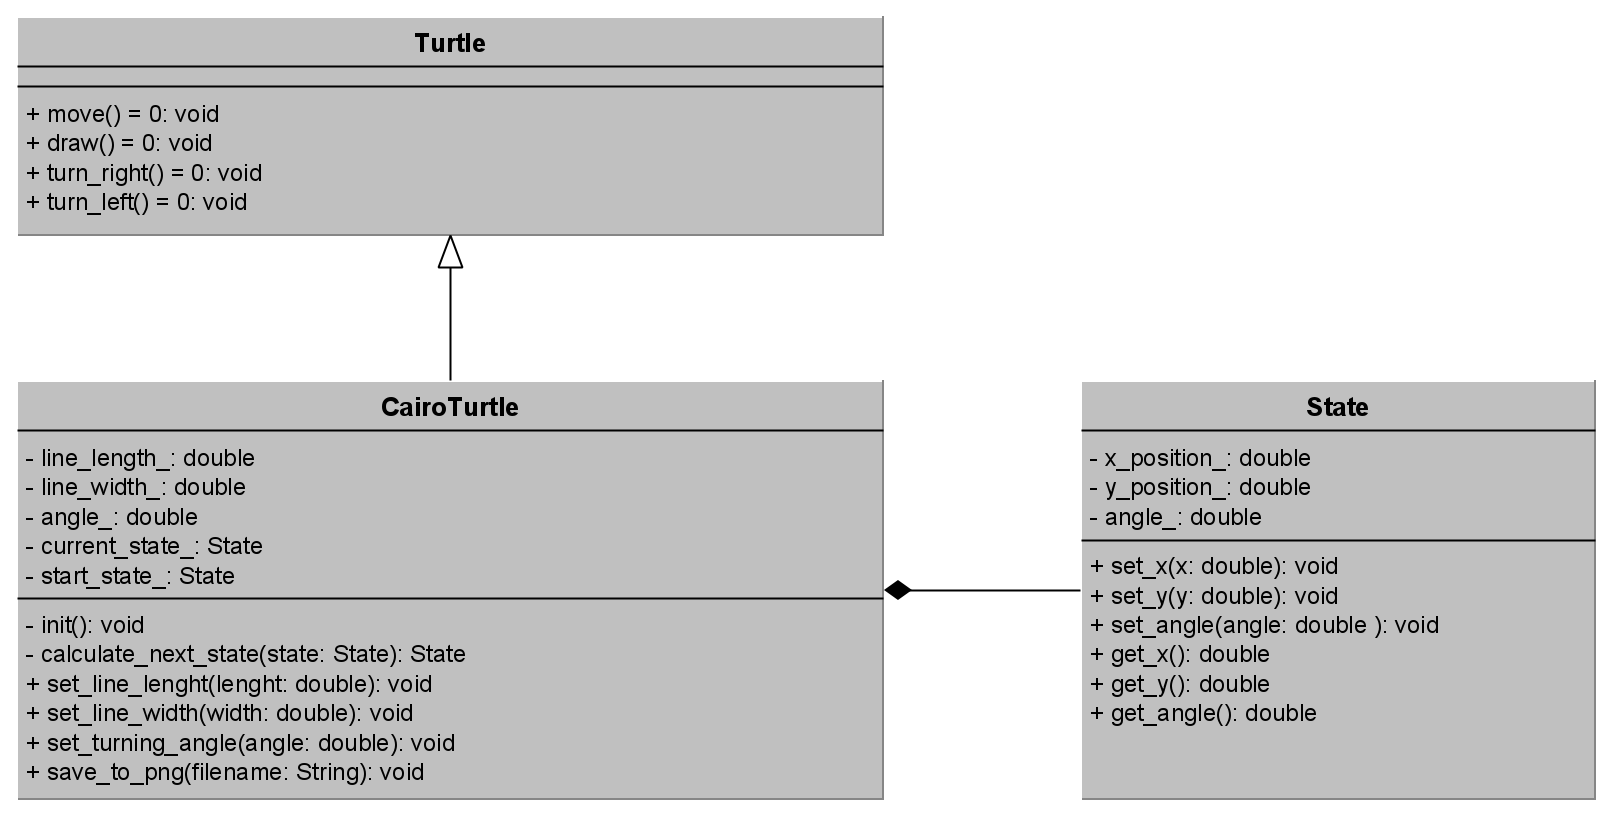
\includegraphics[width=1\columnwidth]{../graphs/LSystem/examples/class_cairo_turtle.png}
	\caption{Cairo turtle concept}
	\label{figure:cairoturtle}
\end{figure}

\noindent In this figure the the conetxt and the surface from Cairo aren't mentioned yet. These objects will be stored as raw pointers, because they will always be used as such. Addtional is the creation and destruction handled by Cairo functions and therefore smartpointers wouldn't add an advantage.\newline

\noindent Cairo offers a function to calculate the bounding box of a recording surface. The function should return the values of an rectangle, including the made draw calls on this surface, but the function didn't return the correct bouding box. In order to get the correct bouding box, an addtional class is introduced - the bounding box. The turtle will hold this class and update it on each draw call. When the save function is called the bounding box will return the size and the translation values to center the graphic for the output file.

\noindent At the moment the turtle allows to draw multiple objects, but there is no possibility to delete previous draw calls. If a second object is drawn with the same turtle instance, both objects will be included in the final image. To prevent this, the reset function is offered, which reinitializes the turtle.

The implementation of the turtle can be found in the provided source code and at my github repository.\footnote{See https://github.com/frozzenshooter/LSystems}

\subsubsection{Further implementations}
The abstract turtle class allows further implementations, for example to export a svg file. This could be also done with the Cairo turtle, by including another export function, but a more lightweight solution would be also possible. For example by directly generating the svg components. Another possible enhancement would be the use of OpenGL and draw in a 3D environment. For this the turtle has to provide further functions, like the rotation around axis. For example by providing the needed transformation matrices. Overall the turtle interface should provide enough flexibility to implement an arbitrary trutle with any graphic framework.

\section{Example usage}
The provided sample code provides a simple example for the already shown examples in section \ref{section:examples}. The example will use the introduced architecture, consiting of the cairo turtle, the command mapping iterator and the L-system with the recursive function. 

\section{Testing}

For the introduced components there are test cases for a C0-coverage. The test cases are defined in an additional executable. The additional executable is also defined with CMake and provides an independent usage of teh test project and the L-system project, containing the examples.

\section{Future enhancements}

The implementation of the different components has the potential of further extensions. Obviously the turtle allows new implementations, for example based on other frameworks. But also the already provided implementation of the Cairo turtle can be improved. For example, it would be possible to add a new function to alter the drawing colors. Another possible enhancment is the scaling of a fractal in the Cairo turtle. At the moment the size of the picture will be determined with the bouding box, but this has the disadvantage, that it can grow to an potential endless size. In order to prevent this it would be possible to use further affine transformations on the data and scale the picture to a upper bound size.

\noindent Another part of the architecture is the L-system itself. The L-system is just a dumb data holder and therefore there is potential to provide further functionality. At the moment the L-system validates, that there is only one production for a predecessor, but it won't check if a generationwith the production is even possible. It would be possible to provide a function, which will check if the provided productions will enable a rewrite of the L-system. 

\noindent A futher enhancement would be additonal test cases. At the moment only a C0 coverage is provided, but further test cases could provide a better testing result.

\noindent Another possible enhancement it the configuration. At the moment the implementation only provides a configuration in the code itself. A way more flexible and convinenent way is the configuration with files. This would make it possible to configure a L-system without a change in code, only by providing such a file. A dynamic configuration can include not only the L-system grammar but also configuration of a turtle and the recursivec function. Such a complete configuration can be done with a file, but should be seperated to maintain the flexibility. A simple solution are key-value pairs, but this has the downside of a bad seperation for the different configuration aspects.

A solution is the use of JSON. This allows the seperation of the configuration for each component. A configuration file contains the JSON-object and allows the dynamic configuration. In order to be able to read the file the architecture can provide another component, reading an input stream and loading the configuration. Afterwards, this component provides the configuration for the other components.

\section{Conclusion}
The introduced architcture enables a flexible use of all introduced components. With the formal restrictions different L-systems can be used and calculated. The iterator supports different ways of use for the result of a L-system, like the graphic generation with a turtle. The turtle enables different implementations and supports therefore all kinds of frameworks. 

\noindent Even with this flexible concept, there are remaining problems. The already mentioned bounding box in the Cairo turtle is only a workaround for the not working function from the Cairo library. This bounding box also doesn't consider the width of the lines and because of that should include a dynamic padding. Another not ideal point is the static configuration of a L-system in teh code as mentioned in the further enhancements. 

\noindent Overall the concept provides a flexible and easy extensible implementaion of L-systems.

\footnote{UML DIAGRAMME NOCHMALS ÜBERARBEITEN - nicht immer wirklcihes uml sondern tw zu sehr abhängig von der Implementierung}
\footnote{would be umformulieren}

\pagebreak
\printbibliography

\end{document}